\documentclass[xcolor=dvipsnames]{beamer} 
\setbeamertemplate{blocks}[rounded][shadow=false]

%!!!!!!!!!!!!!!!!!!!!!!!!!!!!!!!!!!!!!!!!!!!!!!!!!!!!!!!!!!!!!!!!!!!!!!!!!!!!!!!!!!!!!!! TODO TODO TODO TODO TODO TODO TODO TODO TODO TODO TODO TODO TODO 
%referências das imagens e outras coisas que encontrar a mais
%colocar os brain storms
%aqueles letreiro gigantes antes das seções
%Falar quanto o projeto gastou de le até agora
%http://professorcesarcosta.com.br/upload/imagens_upload/nac_08_4.o%20Congresso_ISA.pdf

% CAMPOS, Augusto. O que é Linux. BR-Linux. Florianópolis, março de 2006. Disponível em <http://br-linux.org/faq-linux>. Consultado em [data da sua consulta].

%\usetheme{Boadilla}
%\usetheme{Frankfurt}
\usetheme{Madrid}

\setcounter{tocdepth}{3}
\setcounter{secnumdepth}{3}

\setbeamertemplate{items}[square]
\setbeamertemplate{caption}[numbered]
\usecolortheme{beaver}
\usecolortheme{dolphin}

%todo
\usepackage{xkeyval}
\usepackage{todonotes}
\presetkeys{todonotes}{inline}{}

\usepackage{helvet}
\renewcommand{\familydefault}{\sfdefault}

\usepackage{float}
\usepackage[brazil]{babel}
\usepackage[utf8]{inputenc}

\usepackage{graphicx}
\usepackage{url}
\usepackage{float}     % para forçar a localizaçao das figuras (usando H no posicionamento, =Here)
\usepackage{subfigure}
\usepackage{mathtools} % setas com texto
\usepackage{multicol}
\usepackage{listings}

\usepackage{scalefnt}
\usepackage{ragged2e}
\usepackage{etoolbox, verbatim}


\setcounter{tocdepth}{2}

\lstset{
	numbers=left,
	stepnumber=1,
	numbersep=5pt,
	numberstyle=\small\color{black},
	basicstyle= \scriptsize,
%	keywordstyle=\color{black},
%	commentstyle=\color{black},
%	stringstyle=\color{black},
	tabsize=2
}

\let\olditem=\item% 
\renewcommand{\item}{\olditem \justifying}%

%\usetheme{Antibes}
%\usetheme{Berlin}

\title[Linux \textit{Driver} \textit{Driver} e FPGA]{Implementação de um \textit{Device} \textit{Driver} para Controle de \textit{Hardware} Reconfigurável}
\author[Guimarães, R.L.M.]{\textbf{Orientado:} Rodolfo Labiapari Mansur Guimarães, \\ \textbf{Orientador:} Otávio de Souza Martins Gomes, \\ \textbf{Coorientador:} Diego Mello da Silva.}
\institute[IFMG]{\begin{figure}
			\centering
			\includegraphics[width=0.4\textwidth]{img/logo.jpg}
		\end{figure}}
%\institute[IFMG]{Instituto Federal de Educação, Ciência e Tecnologia de Minas Gerais - Campus Formiga}
\date[\today]{Apresentação dia \today}

\begin{document}


\frame{\titlepage}

\AtBeginSection[] 
{
	\begin{frame}
	\frametitle{Sumário}
	\tableofcontents[]
	\end{frame}
}

\AtBeginSubsection[] 
{
	\begin{frame}
	\frametitle{Sumário}
	\tableofcontents[
    currentsection, 
    currentsubsection, 
    hideothersubsections, 
    %sectionstyle=show/hiden, 
    subsectionstyle=show/shaded, ]
	\end{frame}
}


\section{Objetivo}
%\begin{frame}{}
%	\centering \Huge \color{blue} \textbf{Objetivos}
%\end{frame}
	\begin{frame}{Objetivos}
		\begin{block}{Objetivo Geral}
			\begin{itemize}
				\item \textbf{Pesquisa} e \textbf{Desenvolvimento} de um \textbf{\textit{Driver} em plataforma GNU/Linux} para tornar possível a \textbf{comunicação com um dispositivo externo} ao computador:
				\begin{itemize}
					\item  No qual executa um algoritmo de criptografia simétrica.
				\end{itemize}
			\end{itemize}
		\end{block}
		\bigskip
		\begin{block}{Objetivo Específico}
			\begin{itemize}
				%\item Tornar possível a conexão de um \textit{algoritmo de criptografia simétrico desenvolvido em \textit{hardware}} \textbf{com} o \textit{espaço de usuário} por meio de um \textit{Driver} no Kernel Linunx.
				\item Comunicar por meio do protocolo \textbf{USB}.
				\item Componentes de \textbf{código-fonte aberto} junto com \textbf{\textit{hardware} reconfigurável}.
				\item Descrever uma metodologia para o entendimento e desenvolvimento de um \textit{Driver}.
			\end{itemize}
		\end{block}
	\end{frame}

	%Porque estudar este problema
\section{Justificativa}
%\begin{frame}{}
%	\centering \Huge \color{blue} \textbf{Justificativas}
%\end{frame}
	\begin{frame}{Justificativas}
		%\begin{block}{Objetivo}
			%\item Construir um `sistema' de componentes onde seja possível conectar um dispositivo USB Serial ao espaço do usuário.
			%Construir um \textbf{\it sistema de componentes} onde seja possível conectar um \textit{hardware} reconfigurável ao espaço de usuário utilizando um \textit{Driver} USB Serial.
		%\end{block}
		%\bigskip
		\begin{enumerate}
			\setlength\itemsep{1.5em}
			\item Algoritmos desenvolvido em \textit{hardware} \textbf{necessitam} de uma interface de controle para a comunicação com o usuário.
			%\item Abrangência sobre conhecimento em sistemas operacionais no âmbito:
			%\begin{itemize}
			%	\setlength\itemsep{1em}
			%	\item \textit{Driver} \textit{Driver} dentro de um sistema operacional Linux;
			%	\item Comunicação através de protocolo USB.
			%\end{itemize} 
			%\todo{Porque \textit{Drivers} são genéricos e complexos}
			\item Os \textit{Drivers} atuais são genéricos \cite{corbet2005linux}:
			\begin{itemize}
				\item Tornando suficientemente para serem extremamente complexos.
			\end{itemize}
			\item Documentação sobre desenvolvimento de um \textit{Driver}.
			%\todo{Citar trabalhos relacionados e falar o que o seu é diferente}
			%\todo{Colocar mais coisas}
			%\item - já existe algo feito?
			%\item - porque utilizar o tty ao invés do blocos
				% Creio que no livro ldd deve ter uma explicação pra isso
		\end{enumerate}
	\end{frame}



\section{Metodologia}
	\subsection{Materiais}
%\begin{frame}{}
%	\centering \Huge \color{blue} \textbf{Metodologia} \\[1cm] Materiais
%\end{frame}
	\begin{frame}{Materiais}
		\begin{itemize}
			\item Itens utilizados para a realização da pesquisa:
			\bigskip
			\begin{enumerate}
  				\setlength\itemsep{1em}
				\item \textbf{Dispositivo Lógico Programável:}  FPGA;
%				\item Analisador Lógico Saleae Logic 16;
				\item \textbf{Plataforma de Prototipagem:}  Arduino;
				\item \textbf{Sistema Operacional:} GNU/Linux.
			\end{enumerate}
		\end{itemize}
	\end{frame}




	\subsection{Métodos}
	\begin{frame}{Método - \textit{Software}}
		\begin{multicols}{2}
				%\begin{itemize}
				%	\item Escrita do \textit{Driver}:
					\begin{itemize}
						\item Pesquisa no livro \textbf{Linux Driver Driver 3$^{\circ}$ Edição} disponível gratuitamente para leitura e impressão\footnote{\url{https://www.makelinux.net/ldd3/}.} \cite{corbet2005linux}.
						\item Utilizou-se de \textbf{\textit{mailing lists}} do sítio \url{linux-usb.org} para suprimir dúvidas.
						%https://www.kernel.org/doc/Documentation/driver-model/
						\item Documentação do Linux Kernel\footnote{\url{https://www.kernel.org/doc/Documentation/driver-model/}.}.
						\item Estudo de \textit{Drivers} do Kernels.
					\end{itemize}
				%\end{itemize}
			\columnbreak
				\begin{figure}[p]
					\centering
					\includegraphics[width=0.33\textwidth]{img/livro.jpg}
					\caption{Linux Device Driver 3$^{\circ}$ Edição \cite{corbet2005linux}.}
					\label{fig:ldd3}
				\end{figure}
		\end{multicols}
	\end{frame}

	\begin{frame}{Método - \textit{Hardware}}
		\begin{itemize}
			\setlength\itemsep{2.2em}
			\item Cursos introdutório sobre \textbf{Linguagem VHDL e Sintetização de Projetos em Hardware}.
			%\item Em seguida, com a pesquisa aplicada, aprimorou-se o desenvolvimento de projetos de maior porte e mais complexos.
		\end{itemize}
	\end{frame}
	\begin{frame}{Método}
		\begin{enumerate}
			\setlength\itemsep{1.2em}
			%\begin{itemize}
				%\item A apredizagem e desenvolvimento foram iniciados em projeto de pesquisa aplicada\footnote{ANEXO VI - Edital no 156/2013, protocolo 23208.01490/2013DV.};
			%\end{itemize}
			\item Pesquisa sobre \textbf{desenvolvimento de \textit{Drivers}}:
			\begin{itemize}
				\item Características principais;
				\item Tipos;
				\item Escrita;
				\item Compilação.
			\end{itemize}
			\item FPGA:
			\begin{itemize}
				\item Escrever procedimentos de envio e recebimento de dados;
				\item Máquina de estado controladora.
			\end{itemize}
			\item \textbf{Interconectar} as duas extremidades usando o \textbf{Arduino}.
		\end{enumerate}
	\end{frame}
	\begin{frame}{Método - Estrutura do Projeto}
		\begin{figure}[p]
			\centering
			\includegraphics[width=0.72\textwidth]{img/projeto.png}
			\caption{Representação do projeto numa visão geral.}
			\label{fig:projeto}
		\end{figure}
	\end{frame}











\section{Referencial Teórico}
	\subsection{Materiais}
	\subsubsection{FPGA}
	\begin{frame}{FPGA}
		\centering \color{blue} {\Huge \textbf{FPGA} \\[0.5cm]}% {\huge FPGA}
	\end{frame}
	\begin{frame}{FPGA}
		\begin{itemize}
  			\setlength\itemsep{1em}
		%It consists of an array of logic blocks and routing channels. Two I/O pads fit into the height of one row or the width of one column, as shown below. All the routing channels have the same width (number of wires). 
			\item Tocci (2003) cita que os dispositivos lógicos programáveis são as ``\textit{maravilhas de flexibilidade de projeto}''.
			\item FPGA (\textit{Field Programmable Gate Array}, ou seja, Arranjo de Portas Programável em Campo) consiste num \textbf{arranjo de blocos lógicos} e \textbf{canais de roteamento}.
			\item Significa que é capaz de alterar seus caminhos de dados/fluxos \textbf{habilitando/desabilitando módulos} \cite{moreira2008plataforma}.
		\end{itemize}
	\end{frame}
	\begin{frame}{FPGA - Roteamento de Blocos}
		\begin{figure}[p]
			\centering
			\includegraphics[width=0.55\textwidth]{img/fpga/exemploInicial.png}
			\caption{Exemplo de roteamento interno no FPGA.}
			\label{fig:fpgaHardware}
		\end{figure}
	\end{frame}
	%\begin{frame}{FPGA - Roteamento de Blocos}
	%	\begin{figure}[p]
	%		\centering
	%		\includegraphics[width=0.6\textwidth]{img/fpga/exemplo.jpg}
	%		\caption{Outro exemplo de roteamento interno no FPGA.}
	%		\label{fig:fpgaHardware}
	%	\end{figure}
	%\end{frame}
	\begin{frame}%{FPGA - Roteamento de Blocos}
		\begin{figure}[p]
			\centering
			\includegraphics[width=0.64\textwidth]{img/fpga/exemploFinal.png}
			\caption{Exemplo de roteamento interno bastante complexo no FPGA..}
			\label{fig:fpgaHardware}
		\end{figure}
	\end{frame}
	\begin{frame}{FPGA - Placa}
		\begin{figure}[p]
			\centering
			\includegraphics[width=0.8\textwidth]{img/fpgaHardware.png}
			\caption{FPGA de Desenvolvimento Altera DE2-115.}
			\label{fig:fpgaHardware}
		\end{figure}
	\end{frame}
	\begin{frame}
		\begin{figure}[p]
			\centering
			\includegraphics[width=0.97\textwidth]{img/fpga/altera.png}
			\caption{Altera Quartus II.}
			\label{fig:fpgaHardware}
		\end{figure}
	\end{frame}
	\begin{frame}{FPGA}
		\begin{itemize}
			\item Características importantes da placa utilizada:
			\begin{itemize}
  				\setlength\itemsep{1em}
				\item \textbf{Altera DE2-115} utilizada para ensino e desenvolvimento.
				\item Quantidade de elementos lógicos: 114.480;
				\item IDE\footnote{Integrated Development Environment ou Ambiente de Desenvolvimento Integrado.} Quartus II;
				\item Utilizou-se a linguagem de descrição de \textit{hardware} VHDL;
				\begin{itemize}
					\item \textit{VHSIC Hardware Description Language}, ou seja, uma linguagem de descrição de hardware VHSIC\footnote{\textit{Very High Speed Integrated Circuits.}}.
				\end{itemize}
				\item \textit{Clock} de $50Mhz$;
				\item \textbf{Várias interfaces} para acomodar as mais diversas aplicações.
			\end{itemize} 
			\bigskip
			\item São muito utilizados para \textbf{desenvolver protótipos} e \textbf{realização de testes} antes da fabricação em massa \cite{skliarova2003introduccao}.
		\end{itemize}
	\end{frame}

%	\begin{frame}{Saleae Logic16}
%	\end{frame}

	\subsubsection{Arduino}
	\begin{frame}{Arduino}
		\centering \color{blue} {\Huge \textbf{Arduino} \\[0.5cm]}% {\huge FPGA}
	\end{frame}
	\begin{frame}{Arduino}
		\begin{itemize}
  			\setlength\itemsep{0.8em}
			% http://www.abenge.org.br/CobengeAnteriores/2012/artigos/103723.pdf  pag 3
			\item Plataforma de prototipagem eletrônica aberta baseada em microcontrolador.
			\item Utiliza linguagem de programação Arduino além da IDE Arduino.
			\item Facilidades:
			\begin{itemize}	
  				\setlength\itemsep{0.3em}
				\item \textbf{Reduz} a complexidade da montagem da infraestrutura do projeto;
				\item Possui vários meios de obter informações de uso e sem custo;
				\item É uma plataforma de \textbf{computação física}\footnote{Sistemas digitais podem mensurar variáveis no ambiente físico e tomar decisões sobre tal.}.
			\end{itemize}
			%\item Possui como componentes básicos:
			%\begin{itemize}
  			%	\setlength\itemsep{0.3em}
			%	\item Entrada com \textbf{conversores Analógico-Digital};
			%	\item Entrada e saída de porta digitais;
			%	\item Saída analógica utilizando \textbf{PWM} (\textit{Pulse-Width Modulation});
			%	\item Comunicações;
			%	\item \textbf{Módulos} que podem ser acoplado a ele.
			%\end{itemize} 
		\end{itemize}
	\end{frame}
	\begin{frame}{Arduino Mega 2560}
		\begin{figure}[p]
			\centering
			\includegraphics[width=0.9\textwidth]{img/arduino/arduinomega.jpg}
			\caption{Arduino Mega 2560.}
			\label{fig:arduinoHardware}
		\end{figure}
	\end{frame}
	\begin{frame}%{IDE Arduino 1.6.5}
		\begin{figure}[p]
			\centering
			\includegraphics[width=0.72\textwidth]{img/arduino/ide.png}
			\caption{IDE Arduino 1.6.5.}
			\label{fig:arduinoHardware}
		\end{figure}
	\end{frame}
	\begin{frame}{Arduino}
		\begin{itemize}
			\item Características do Arduino utilizado no trabalho:
			\bigskip
			\begin{itemize}
  				\setlength\itemsep{0.9em}
				\item \textbf{Arduino Mega 2560} com microcontrolador ATmega2560;
				\item Possui 54 portas de entrada e saída Digital:
				\begin{itemize}
					\item Sendo 15 podendo ser utilizadas para saída PWM (\textit{Pulse-Width Modulation}).
				\end{itemize}
				\item Outras 16 portas para entrada analógica;
				\item Frequência de \textit{Clock} de $16 MHz$.
				%\item Memória?
			\end{itemize} 
		\end{itemize}
	\end{frame}


	\subsubsection{Linux}
	\begin{frame}{Linux}
		\centering \color{blue} {\Huge \textbf{Linux} \\[0.5cm]}% {\huge FPGA}
	\end{frame}
	% https://pt.wikipedia.org/wiki/Linux
	\begin{frame}{Linux}
		\begin{itemize}
			\setlength\itemsep{0.9em}
			\item \textbf{Linux} é um termo utilizado para referir sistemas operacionais que utilizam o \textbf{kernel Linux}.
			\item O sistema operacional como um todo tem como nome \textbf{GNU/Linux}. 
			\item Linux Kernel foi desenvolvido por Linus Torvalds em 1991.
			\item Reimplementação reelaborada do MINIX\footnote{Baseado no UNIX.} obedecendo o padrão POSIX \cite{nemeth2004manual}.
			\item Hoje é desenvolvido/estudado em projetos colaborativos de código-fonte aberto com principalmente:
			\begin{itemize}
				\setlength\itemsep{0.5em}
				\item Programadores individuais/Entusiastas;
				\item Colaborações de grandes empresas como \textit{IBM, Sun Microsystems, HP, Oracle, Google}, entre outras.
			\end{itemize}
		\end{itemize}
	\end{frame}
	\begin{frame}{Linux}
		\begin{itemize}
			\setlength\itemsep{1em}
			%\item Qualquer pessoa pode utilizar, estudar, modificar e distribuir o sistema segundo a licensa GPL\footnote{Executar e modificar desde que ajude ao seu próximo.}.
			\item Linux é um kernel \textbf{monolítico} no qual os \textit{Drivers} podem:
			\begin{itemize}
				\setlength\itemsep{0.7em}
				\item Executar com acesso total ao \textit{hardware};
				\item Configurados como módulos e carregados/descarregados \textbf{enquanto o sistema está ligado}.
			\end{itemize}
			\item Executa em arquiteturas como: \textit{Intel, StrongARM, PowerPC, Alpha}, etc. além de embarcados.
			\item Hoje, é possível encontrar distribuições Linux com coleções de \textit{software} (por exemplo o GNU) pronto para o uso \cite{campos}.
			%\item Uma das vantagens do sistema operacional livre é que seus módulos estão disponíveis para estudo.
			%\item Escrever um programa em espaço de usuário para torna-se mais fácil com uso de um \textit{Driver}.
		\end{itemize}
	\end{frame}
	\begin{frame}{Linux}
		\begin{multicols}{2}
				A distribuição Linux utilizada para a realização do desenvolvimento:
				\bigskip
				\begin{itemize}
					\item \textbf{Linux Mint 17.2} com codinome Rafaela, 64-bits;
				\end{itemize}
				\begin{figure}[p]
					\centering
					\includegraphics[width=0.27\textwidth]{img/linux/mint.jpg}
					\caption{Logo Linux Mint.}
					\label{fig:mint}
				\end{figure}
			\columnbreak
				Sendo executado na máquina virtual:%
				\bigskip
				\begin{itemize}
					\item \textbf{Oracle VM VirtualBox 5.0.8} instalada no OS X El Capitan.
				\end{itemize}
				\begin{figure}[p]
					\centering
					\includegraphics[width=0.25\textwidth]{img/linux/vm.png}
					\caption{Logo Oracle VM VirtualBox.}
					\label{fig:vb}
				\end{figure}
		\end{multicols}
	\end{frame}



	\subsection{Protocolos}
	\begin{frame}{Comunicação Serial}
		\begin{itemize}
			\setlength\itemsep{2.2em}
			\item Utilizadas a mais de 40 anos para a comunicação entre dispositivos \cite{nemeth2004manual}.
			\item São representadas por arquivos de dispositivo no diretório \texttt{ /dev}.
			%\begin{itemize}
			%	\item O nome dos arquivos é relevante somente para o usuário. O mapeamento é determinado pelos números Major e Minor.
			%\end{itemize}
			\item Foram utilizados dois protocolos de comunicação serial sendo eles:
			\begin{itemize}
				\setlength\itemsep{1em}
				\item UART;
				\item USB.
			\end{itemize}
		\end{itemize}
	\end{frame}
	\begin{frame}{Protocolos - UART}
		\begin{itemize}
			\item \textit{\textbf{U}niversal \textbf{A}synchronous \textbf{R}eceiver/\textbf{T}ransmitter}.
		\end{itemize}
		\bigskip
		\begin{figure}[p]
			\centering
			\includegraphics[width=1\textwidth]{img/fpga/uart.png}
			\caption{Protocolo de comunicação UART.}
			\label{fig:uart}
		\end{figure}
	\end{frame}
	\begin{frame}{Protocolos - USB}
	%\todo{Rever esse slide pra que fique mais fácil o entendimento}
		\begin{itemize}
			\setlength\itemsep{1em}
			\item \textbf{Atributos:} \textit{idVendor}, \textit{idProduct}, Números de \textit{Interfaces}, \textit{Endpoints}...
			\item \textbf{Um dispositivo USB possui:} \textit{Configurations}, \textit{Interfaces} e \textit{Endpoints}.
			\item Modo de envio de pacotes \textbf{por meio (ou não)} de \textbf{URB\footnote{\textit{\textbf{U}SB \textbf{R}equest \textbf{B}lock}.}}:
			\begin{itemize}
				\setlength\itemsep{0.7em}
				\item \textbf{Tipo:} Interrupt, Bulk, Control, Isochronous;
				\item \textbf{Operações:} Criar, destruir, enviar, callback handler, cancelamento.
			\end{itemize}
			\item Entre muitas outras características.
		\end{itemize}
	\end{frame}
	\begin{frame}
		\begin{figure}[p]
			\centering
			\includegraphics[width=0.87\textwidth]{img/endpoint2.png}
			\caption{Exemplo de comunicação USB.}
			\label{fig:uart}
		\end{figure}
	\end{frame}
	\begin{frame}{Protocolos - USB}
		\begin{itemize}
			\setlength\itemsep{1em}
			\item \textbf{Vantagens:}
			\begin{itemize}
				\setlength\itemsep{0.7em}
				\item \textit{Universal Serial Bus} é um sistema de \textbf{interconexão de periféricos genéricos}.
				\item \textbf{Cabos e conectores padronizados} além de vários \textbf{adaptadores} para extender suas funcionalidades.
				\item É um excelente sistema e que acredita-se durar ainda por vários anos \cite{nemeth2004manual}.
				\item O Linux tem um \textbf{amplo e sólido suporte} ao USB.
			\end{itemize}
			\item \textbf{Desvantagem:}
			\begin{itemize}
				\item Protocolo complexo.
			\end{itemize}
		\end{itemize}
	\end{frame}
	\begin{frame}{\textit{Driver} TTY}
		\begin{itemize}
			\item Abreviatura de \textit{\textbf{t}ele\textbf{t}\textbf{y}pewriter}.
			\item Interligava um terminal (físico ou virtual) a uma máquina Unix.
			\item Meio de nomear qualquer dispositivo de porta serial \cite{corbet2005linux}:
			\begin{itemize}
				\item \textbf{Físicos:}
				\begin{itemize}
					\item Portas Seriais;
					\item Conversores USB/serial;
					\item \textit{Modems} que necessitam de um processamento especial.
				\end{itemize}
				\item \textbf{Virtuais:}
				\begin{itemize}
					\item Consoles virtuais utilizados para fazer login em um computador por meio de uma conexão de rede;
					\item Entre outros.
				\end{itemize}
			\end{itemize}
			\item Vive \textbf{sob} o \textit{Driver} de Caractere e oferece \textbf{recursos de interface}:
			\begin{itemize}
				\item Controla o fluxo de dados;
				\item Formato dos dados.
			\end{itemize}
			\item Foco na \textbf{trasmissão e recebimento de dados com o \textit{hardware}}:
			\begin{itemize}
				\item Ao invés da interação com o espaço do usuário.
			\end{itemize}
		\end{itemize}
	\end{frame}
	\begin{frame}{\textit{Driver} TTY}
		%http://www.linusakesson.net/programming/tty/
		\begin{itemize}
			\item O \textbf{\textit{Driver} TTY}:
			\begin{itemize}
				\item Não comunica diretamente com o TTY \textit{Line Discipline};
				\item Formata os dados pro envio ao \textit{hardware} e também os recebe.
			\end{itemize}
			\item \textbf{TTY \textit{Line Discipline}}:
			\begin{itemize}
				\item Formatar os dados recebidos pelo usuário ou o \textit{hardware}, de forma específica (PPP, Bluetooth por exemplo).
			\end{itemize}
		\end{itemize}
		\begin{figure}[p]
			\centering
			\includegraphics[width=0.85\textwidth]{img/tty.png}
			\caption{Comunicação utilizando TTY.}
			\label{fig:tty}
		\end{figure}
	\end{frame}




\section{Desenvolvimento}
	\subsection{FPGA}
	\begin{frame}{Desenvolvimento - FPGA}
		\centering \color{blue} {\Huge \textbf{FPGA} \\[0.5cm]}% {\huge FPGA}
	\end{frame}
	\begin{frame}{Desenvolvimento - FPGA}
		\begin{itemize}
			\item Síntese do algoritmo \textbf{3DES}, no qual utiliza:
			\begin{itemize}
				\item \textbf{Três chaves de 64-\textit{bits}};
				\item \textbf{Blocos de texto de 64-\textit{bits}}.
			\end{itemize}
			\bigskip
			\item Escrita do método de \textbf{envio e recebimento de informações} utilizando protocolo \textbf{UART}\footnote{\textit{\textbf{U}niversal \textbf{A}synchronous \textbf{R}eceiver/\textbf{T}ransmitter}}:
		\end{itemize}
		\begin{figure}[p]
			\centering
			\includegraphics[width=1\textwidth]{img/fpga/uart.png}
			\caption{Protocolo de comunicação UART.}
			\label{fig:uart}
		\end{figure}
	\end{frame}
	\begin{frame}{Desenvolvimento - FPGA - Máquina de Estados Controladora}
		\begin{figure}[p]
			\centering
			\includegraphics[width=1\textwidth]{img/fpga.png}
			\caption{Exemplo da máquina de Estados do FPGA.}
			\label{fig:mefpga}
		\end{figure}
	\end{frame}


	\subsection{Linux}
	\begin{frame}{Desenvolvimento - Linux}
		\centering \color{blue} {\Huge \textbf{Linux} \\[0.5cm]}
	\end{frame}
	\begin{frame}{Desenvolvimento - Linux}
		\begin{itemize}
			\setlength\itemsep{2em}
			%\item Entendido como compila e carrega um \textit{Driver} ao Kernel, iniciou-se o estudo de desenvolvimento.
			%item Após estudado todas possibilidades de desenvolvimento 
			\item Percebeu-se que existe \textbf{3 classes} de um \textit{Driver} genérico:
			\begin{itemize}
				\setlength\itemsep{1em}
				\item \textbf{Bloco:} 512 \textit{bytes} ou maiores, em potência de 2, mapeado em \texttt{/dev};
				\item \textbf{Interface de Rede:} tratamento de pacote de redes, mapeado como \texttt{eth0};
				\item \textbf{Caractere:} mapeado em \texttt{/dev}.
			\end{itemize}
			\item De todos, o \textit{Driver} pertencentes à classe Caracteres mostrou-se mais \textbf{simples} e \textbf{eficaz} para a comunicação USB.
			%\item Os módulos são desenvolvidos em linguagem C porém com bibliotecas do próprio Kernel.
			%\begin{itemize}
			%	\item \texttt{printf()} por \texttt{printk()};
			%	\item \texttt{malloc()} por \texttt{kalloc()};
			%	\item Entre outros.
			%\end{itemize}
		\end{itemize}
	\end{frame}
	\begin{frame}{Desenvolvimento - Linux}
		\begin{itemize}
			\setlength\itemsep{2em}
			\item Com pesquisas mais profundas, descobriu-se que:
			\begin{itemize}
				\setlength\itemsep{1em}
				\item Unir a comunicação {\bf TTY} (\textit{Driver Char}) com bibliotecas do Kernel específicas para USB torna a escrita mais facilitada;
			\end{itemize}
			%\item Assim, o \textit{Driver} não seria somente um \textit{Driver} de comunicação de caracteres, mas sim com a facilidade do TTY;
			\item Utilizado o TTY com a biblioteca USB Serial:
			\begin{itemize}
				\setlength\itemsep{1em}
				\item Utilizar \textbf{Macros} tornando o processo automatizado;
				\item O \textbf{desenvolvimento} é facilitado;
				\item E consequentemente a \textbf{compreensão}.
			\end{itemize}
			%\item O suporte do \textit{Driver} é descrito numa tabela de dispositivos:
			%\begin{itemize}
			%	\item idVendor, idProduct, ou a classe do dispositivo.
			%\end{itemize}
			%\item Comunicação por meio do diretório \texttt{/dev/tty}
		\end{itemize}
	\end{frame}
	\begin{frame}{Comunicação utilizando TTY}
		%http://www.linusakesson.net/programming/tty/
		\begin{figure}[p]
			\centering
			\includegraphics[width=1\textwidth]{img/tty.png}
			\caption{Comunicação utilizando TTY.}
			\label{fig:tty}
		\end{figure}
	\end{frame}


	\subsection{Arduino}
	\begin{frame}{Desenvolvimento - Arduino}
		\centering \color{blue} {\Huge \textbf{Arduino} \\[0.5cm]}
	\end{frame}
	\begin{frame}{Desenvolvimento - Arduino}
		\begin{itemize}
			\setlength\itemsep{2em}
			\item \textbf{Função:} Interconectar o FPGA com o \textit{Driver}.
			\begin{enumerate}
				\setlength\itemsep{1em}
				\item O FPGA não tem interface `\textit{amigável}' para o usuário;
				\item E o \textit{Driver} só realiza a comunicação entre o espaço do usuário com o \textit{hardware}.
			\end{enumerate}
			\item Possui uma máquina de estados no qual:
			\begin{itemize}
				\setlength\itemsep{1em}
				\item \textbf{Controla} as informações a serem exibidas para o usuário;
				\item \textbf{Instrui} quais passos podem ser executados nos momentos certos;
				\item \textbf{Armazena} as informações para operação de forma organizada.
			\end{itemize}
		\end{itemize}
	\end{frame}
	\begin{frame}{Desenvolvimento - Estrutura do Projeto}
		\begin{figure}[p]
			\centering
			\includegraphics[width=0.72\textwidth]{img/projeto.png}
			\caption{Representação do projeto numa visão geral.}
			\label{fig:projeto}
		\end{figure}
	\end{frame}



%	\begin{frame}{Desenvolvimento - Arduino}
%		\begin{itemize}
%			\item As antigas e as novas (o quão simplificadas elas são em relação às antigas)
%			\item 
%		\end{itemize}
%		\begin{itemize}
%			\item Deixar claro o qur foi feito no FPGA, o que foi feito no Arduino, linguagens utilizadas
%		\end{itemize}
%	\end{frame}




	%Porque estudar este problema
\section{Conclusão}
%\begin{frame}{}
%	\centering \Huge \color{blue} \textbf{Justificativas}
%\end{frame}
	\begin{frame}{Tarefas Cumpridas}
		\begin{enumerate}
			\item \textbf{\textit{Driver}:}
			\begin{itemize}
				\item Concede a comunicação com o Arduino via USB por meio de funções de manipulação de arquivos situados no diretório {\tt /dev}.
			\end{itemize}
			\item \textbf{Arduino:} 
			\begin{itemize}
				\item Realiza seu papel de intermediário entre as extremidades:
				\begin{itemize}
					\item Tanto com o FPGA quanto com o \textit{Driver}.
				\end{itemize}
				\item Exibe as informações corretamente.
			\end{itemize}
			\item \textbf{FPGA:}
			\begin{itemize}
				\item É possível realizar a encriptação de \textbf{apenas 1 bloco de 64-bits por vez}:
				\begin{itemize}
					\item Sendo este alterado manualmente pelo usuário.
				\end{itemize} 
			\end{itemize}

			%\begin{itemize}
			%	\item \textit{Driver} \textit{Driver} dentro de um sistema operacional Linux;
			%	\item Comunicação através de protocolo USB;
			%\end{itemize} 
			%\item Desenvolver um \textit{Driver} simples e de fácil entendimento.
		\end{enumerate}
	\end{frame}
	\begin{frame}{Exemplo Prático}
		\begin{figure}[p]
			\centering
			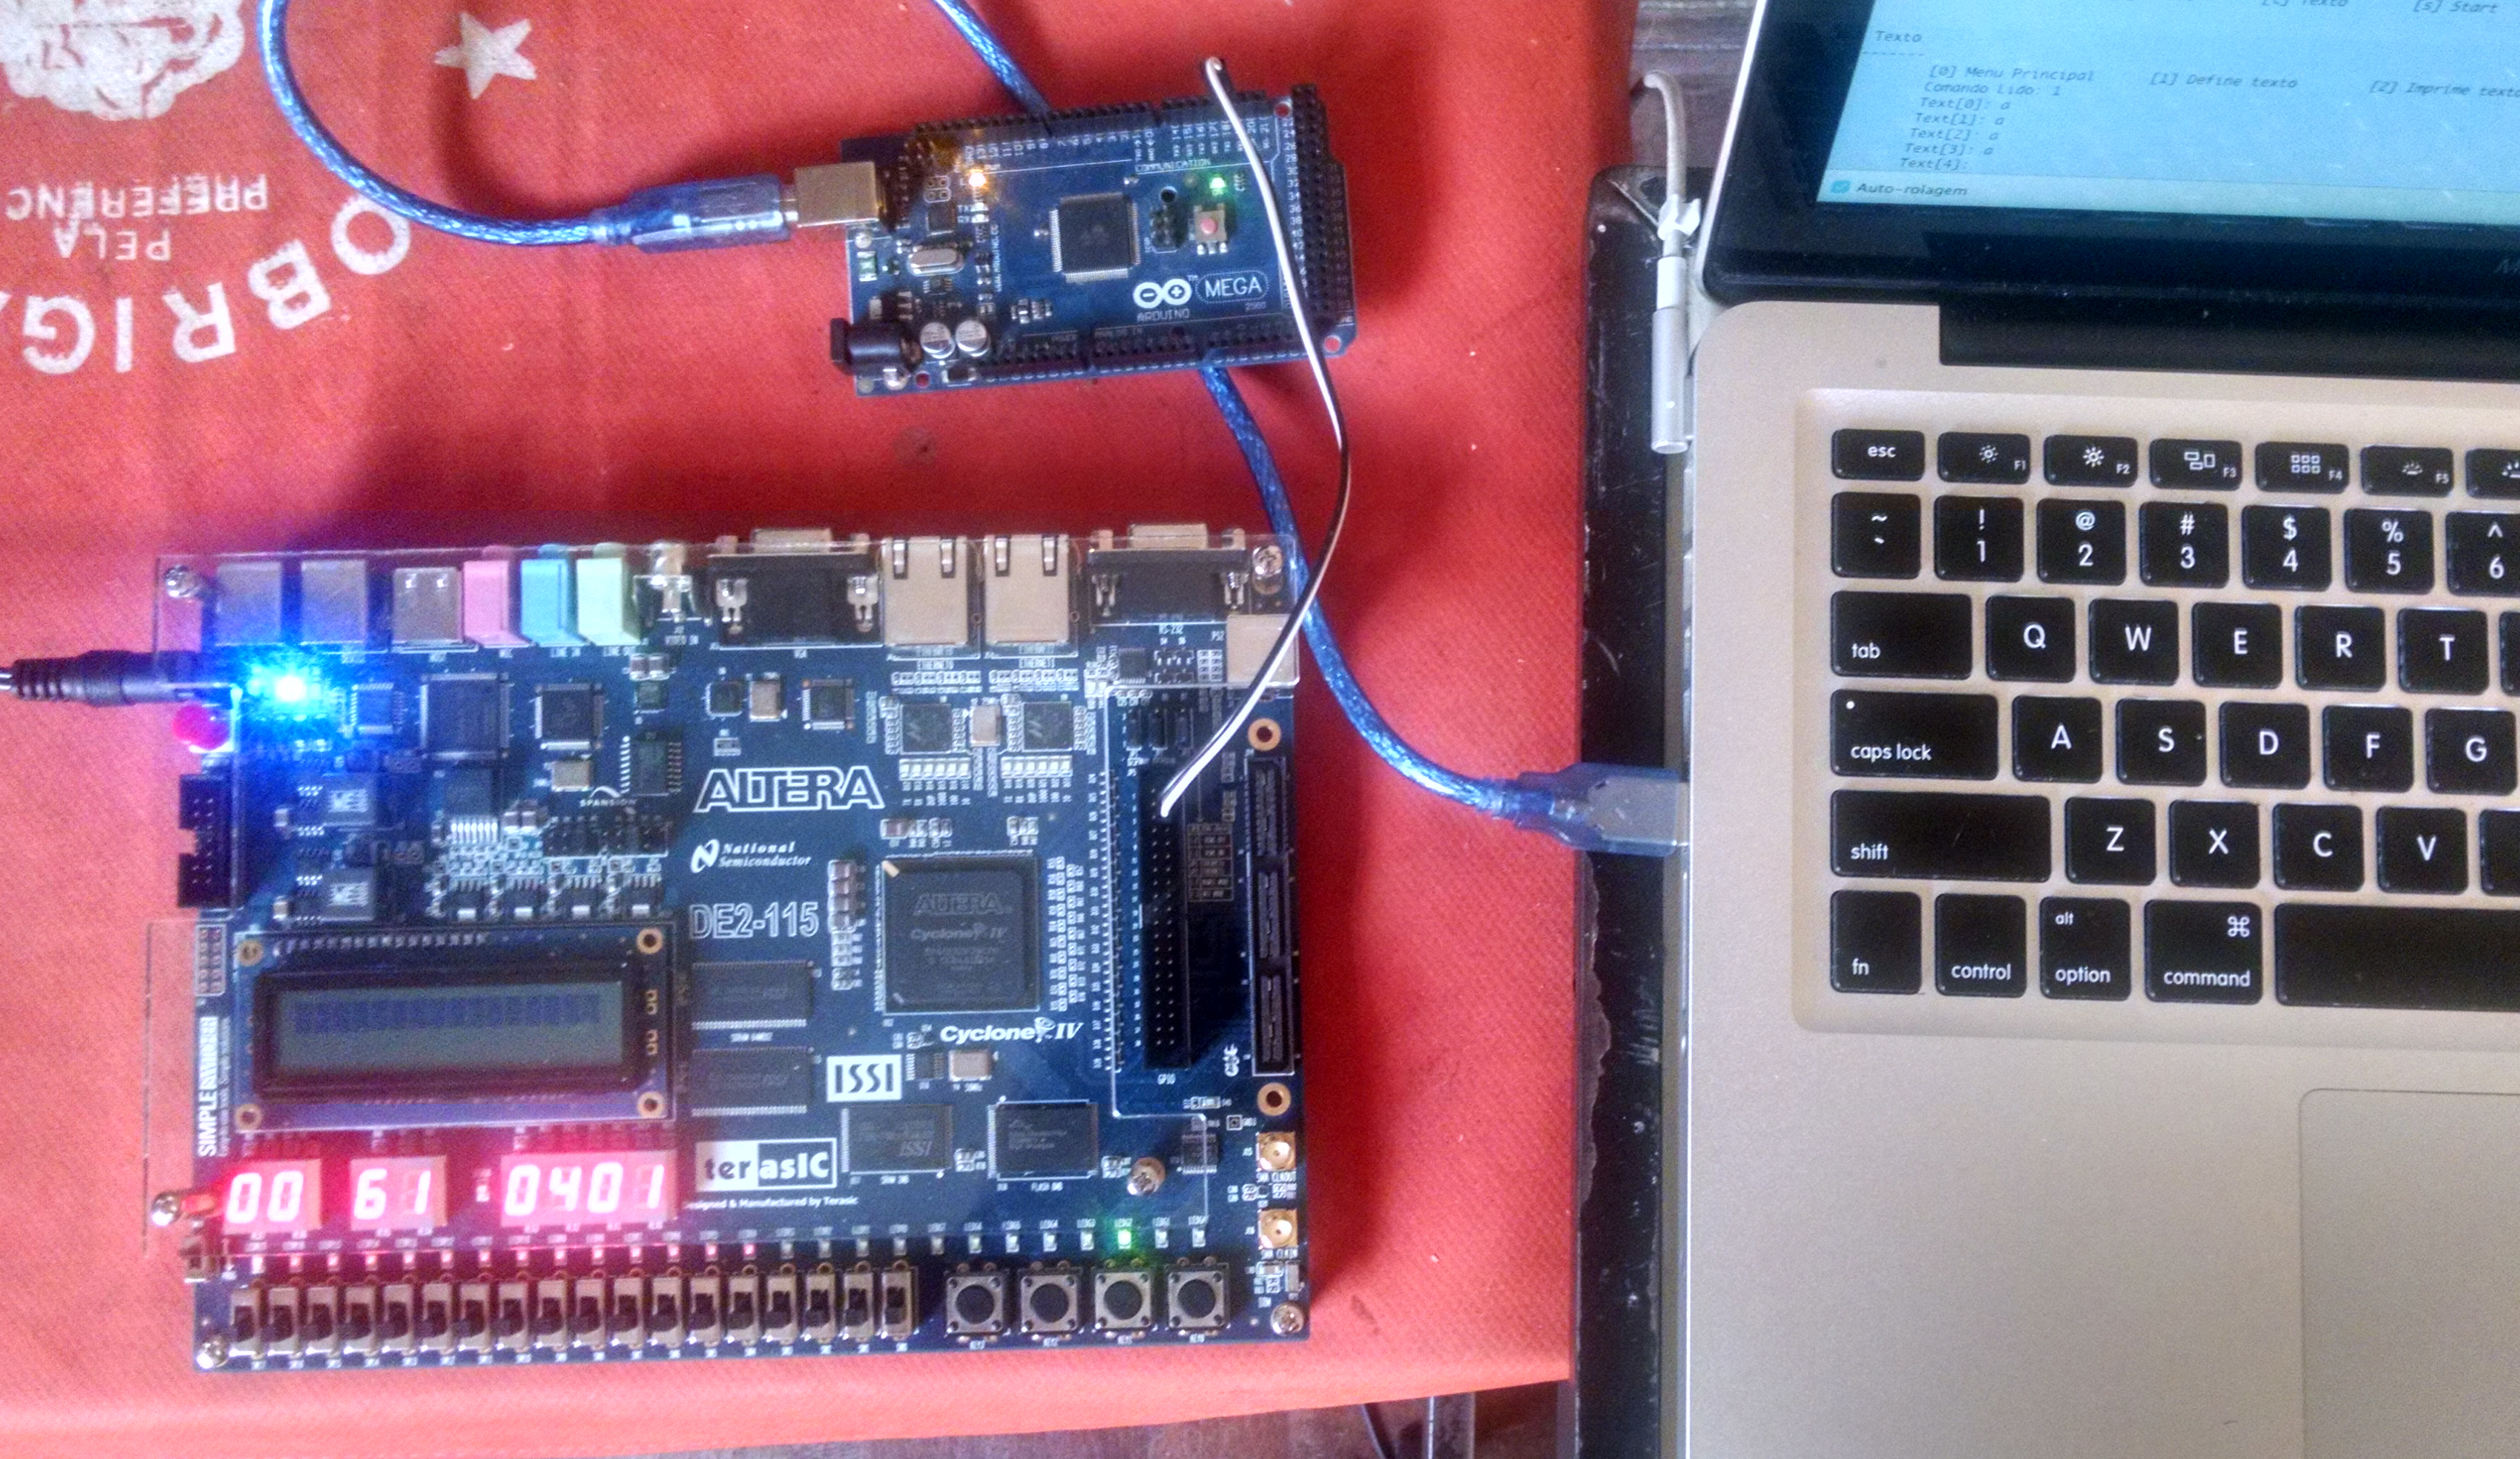
\includegraphics[width=1\textwidth]{img/projetoReal/real.jpg}
			\caption{Foto real do projeto em atuação.}
			\label{fig:projetoreal}
		\end{figure}
	\end{frame}
	\begin{frame}{Tarefas Pendentes}
		\begin{enumerate}
			\item Além da \textbf{encriptação}, adicionar o algoritmo que realiza a \textbf{decodificação}:
			\begin{itemize}
				\item Adicionar os procedimentos pra que a decriptação seja possível.
			\end{itemize}
			\item Atualmente encripta-se somente 1 bloco por vez (alterado manualmente pelo usuário):
			\begin{itemize}
				\item Permitir que o envie o texto do tamanho que quiser desde que:
				\begin{itemize}
					\item Seu limite seja a capacidade de armazenamento interno do Arduino.
				\end{itemize}
			\end{itemize}
			\item Desenvolver um conhecimento maior para aprimorar o \textit{Driver} TTY.

			%\begin{itemize}
			%	\item \textit{Driver} \textit{Driver} dentro de um sistema operacional Linux;
			%	\item Comunicação através de protocolo USB;
			%\end{itemize} 
			%\item Desenvolver um \textit{Driver} simples e de fácil entendimento.
		\end{enumerate}
	\end{frame}

\begin{frame}[allowframebreaks]
        \frametitle{Referências}
		\bibliographystyle{abnt}
        \bibliography{referencias.bib}
\end{frame}

\frame{\titlepage}


\section*{Extra}

	\begin{frame}{Projetos Futuros}
		\begin{itemize}
			\item Alterar o funcionamento da comunicação USB para que tenha uma via só para envio de controle e outra só para envio de dados\footnote{Se possível}.
			\item Adicionando o protocolo USB no FPGA:
			\begin{itemize}
				\item Mensagens de informações ao usuário deverão ser trabalhadas no próprio \textit{Driver} eliminando o dispositivo intermediário\footnote{Hipótese.}; ou
				\item Criação de um \textit{software} a nível de usuário para todo o controle do \textit{hardware}.
			\end{itemize}  
		\end{itemize}
	\end{frame}




		\begin{frame}{FPGA -  Implementações}
			\begin{enumerate}
				\item Algoritmo 3DES de criptografia simétrico desenvolvido em hardware onde:
				\begin{itemize}
					\item 3 chaves de 64 bits (o mesmo que 8 caracteres ASCII de 8 bits);
					\item Texto formado em blocos de 64 bits completos.
				\end{itemize}
				\item Algoritmos de envio e recebimento de dados através de UART.
				\begin{itemize}
  					\setlength\itemsep{.8em}
					\item $Clock_{FPGA} = 50.000.000 \quad\quad Clock_{requerido} = 9.600 $
					\item Cada intervalo teria: $\frac{50.000.000}{9.600} = 5.208,33333~$ clocks do $Clock_{FPGA}$
					\item Ou seja, a cada $ 5.208,33333~$ pulso de clock de $50Mhz$, deve pular 1 do $ NovoClock_{FPGA} $.
					%\item Entretanto, é um número \textit{fracionário} criando uma margem de erro que \textit{pode ser} notável assintoticamente.
					\item Erro: $\frac{|Clk_{Experi} - Clk_{Correto}|}{Clk_{Correto}} = \frac{0,333~}{5.208,0} = 0,06400409626\% $
				\end{itemize}
				\item Máquina de estados controladora do sistema em hardware.
			\end{enumerate}
		\end{frame}


		\begin{frame}{Linux - Detalhes importantes do device driver}
			\begin{itemize}
				\item Então, o `novo' driver possui:
				\begin{itemize} 
					\item Macro de inicialização (\texttt{init(), exit(), probe(), disconnect()});
					\item Funções de envio de pacotes;
					\item Funções como \texttt{open()} e \texttt{close()} para a inicialização e términdo da comunicação;
					\item Uma tabela de devices para possíveis conexões.
				\end{itemize}
				\item E deixou de existir:
				\begin{itemize}
					\item \texttt{Init()};
					\item \texttt{Exit()};
					\item \texttt{Probe()};
					\item \texttt{Disconnect()}...
				\end{itemize}
			\end{itemize}
		\end{frame}

	\begin{frame}[fragile, allowframebreaks]{Complementar}
		\begin{comment}
		\begin{block}{Por que o processamento não fica todo no FPGA?}
			Por ser um hardware extremamente rápido, este ficará exercendo sua função de forma \textbf{dedicada}. Ou seja, se determinado usuário quiser trocar o algoritmo na FPGA, basta ele colocar o novo algoritmo desde que ele funcione por meio de blocos.
		\end{block}

		\begin{block}{Por que não desenvolveu um software em espaço de usuário mais bonito ou funcional? Nem sequer falou de espaço do usuário...}
			O foco do desenvolvimento deste trabalho é justamente a conexão do Kernel ao FPGA. Qualquer software em nível de usuário será tido como trabalho extra.
		\end{block}

		\begin{block}{Poderia ter feito num FPGA com tamanho menor?}
			Sim. Tentou-se desenvolver os algoritmos num Ciclone II, entretanto, este só suporta cerca de 4 mil EL. Então utilizou-se o Ciclone IV disponibilizado pelo IFMG - Formiga que possui cerca de 115 mil.
		\end{block}
		\end{comment}

		\begin{block}{Como é o envio de um URB?}
			\begin{enumerate}
				\item No driver, associa um específico endpoint a um específico device.
				\item Envia do driver para o USB Core
				\item Envia do USB Core para um específico driver Host  Controlardor USB.
				\item Este driver Host Controlador processa essa informação e envia para o device.
				\item Quando o envio é completado, o driver Controlador Host notifica o driver do desenvolvedor.
			\end{enumerate}
		\end{block}

		\begin{block}{Major e Minor Numbers}
			\begin{itemize}
				\item Drivers de Char possuem dois números como parte de suas careacterísticas.
				\begin{itemize}
					\item \textbf{Major:} Identifica que o driver está associado com o device.
					\item \textbf{Minor:}
				\end{itemize}
				\item Por exempo o \texttt{/dev/null} e \texttt{/dev/zero}:
				\begin{itemize}
					\item Ambos tem o número Major igual;
					\item Ele é utilizado para associar o driver ao dispositivo;
					\item Entretanto, possuim o número Minor diferentes.
					\item É usado pelo quernel para determinar qual device específico ele está referenciando.
					\item ...
				\end{itemize}
			
			\end{itemize}
		\end{block}

		\begin{block}{Device}
			\begin{itemize}
				\item Endpoints:
				\begin{itemize}
				    \item Control, Interrupt, Bulk e Isochronous.
				\end{itemize}
				\item Interfaces:
				\begin{itemize}
				    \item Mouse, Teclado possuem somente 1 via;
				    \item Podem ter configurações diferentes;
				    \item Áudio em Linux, por exemplo teria 2 interfaces (Áudio e Controle).
				\end{itemize}
				\item Configurations:
				\begin{itemize}
				    \item Em Linux, não é comum utilizar mais que 1 configuração no dispositivo.
				\end{itemize}
				\item Ou seja:
				\begin{enumerate}
				    \item Devices usually have one or more configurations.
				    \item Configurations often have one or more interfaces.
				    \item Interfaces usually have one or more settings.
				    \item Interfaces have zero or more endpoints.
				\end{enumerate}
			\end{itemize}
		\end{block}


		\begin{comment}
		\begin{block}{Compilação e Execução} 
			\begin{itemize}
				\item Deve compilar o código utilizando um compilador fornecido e integrado no Kernel:
				\begin{itemize}
					\item
				\end{itemize}
				\item Após a compilação...:
				\begin{itemize}
					\item
				\end{itemize}
			\end{itemize}
		\end{block}
		\end{comment}
\end{frame}










	\subsection*{Linguagens de Programação}
	\begin{frame}[fragile]{Linguagens de Programação - VHDL}
		\begin{itemize}
			\item \textit{\textbf{V}HSIC (Very High Speed Integrated Circuits) \textbf{H}ardware \textbf{D}escription \textbf{L}anguage}.

		\begin{lstlisting}[language=VHDL]
-- importa std_logic da IEEE library
library IEEE;
use IEEE.std_logic_1164.all;

-- Declara uma entidade
entity ANDGATE is
   port ( 
         IN1 : in std_logic;
         IN2 : in std_logic;
         OUT1: out std_logic);
end ANDGATE;
architecture RTL of ANDGATE is

begin
  OUT1 <= IN1 and IN2;
end RTL;
		\end{lstlisting}
		\end{itemize}
\end{frame}
	\begin{frame}[fragile]{Linguagens de Programação - Arduino}
	\begin{itemize}
		\item Linguagem Arduino.
		\begin{lstlisting}[language=C++]
// the setup function runs once when you press reset or power the board
void setup() {
  // initialize digital pin 13 as an output.
  pinMode(13, OUTPUT);
}

// the loop function runs over and over again forever
void loop() {
  digitalWrite(13, HIGH);  // turn the LED on (HIGH is the voltage level)
  delay(1000);             // wait for a second
  digitalWrite(13, LOW);   // turn the LED off by making the voltage LOW
  delay(1000);             // wait for a second
}			
		\end{lstlisting} 
	\end{itemize}
\end{frame}

	\begin{frame}[fragile]{Compilação do Driver}
			\begin{lstlisting}
obj-m	:= usbSerial.o

KERNELDIR ?= /lib/modules/$(shell uname -r)/build
PWD       := $(shell pwd)

all:
	rm -f *.o *~ core .depend .*.cmd *.ko *.mod.c *.symvers *.order     
	#sudo /usr/sbin/ntpdate ntp.on.br time.nist.gov pool.ntp.org

	# Compilando os arquivos atraves do kernel
	$(MAKE) -C $(KERNELDIR) M=$(PWD)     
	
	# Copiando para a pasta temporaria
	sudo cp usbSerial.ko /tmp/        
	
	sudo rmmod usbSerial             # Removendo o driver antigo
	
	sudo insmod /tmp/usbSerial.ko    # Adicionando o novo driver
			\end{lstlisting}
\end{frame}



\frame{\titlepage}
\end{document}